\question{Криволинейные интегралы 1-го и 2-го рода: формула связи.}

\begin{twocolumns}
  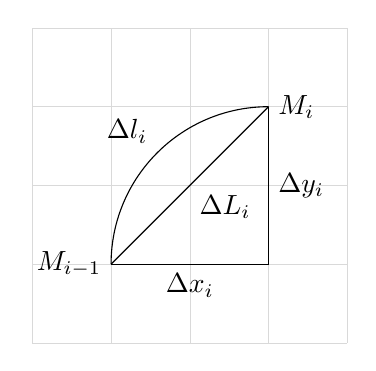
\begin{tikzpicture}  
  \draw[very thin, gray!30, step = 1cm] (0, 0) grid (4, 4);
  \draw (1, 1) -- (3, 1) -- (3, 3);
  \draw (3, 3) arc (90:180:2) node[midway, above left] {\(\Delta l_{i}\)};
  \draw (1, 1) -- (3, 3) node[midway, below right] {\(\Delta L_{i}\)};

  \draw node[below] at (2, 1) {\(\Delta x_{i}\)};
  \draw node[right] at (3, 2) {\(\Delta y_{i}\)};
  \draw node[left] at (1, 1) {\(M_{i - 1}\)};
  \draw node[right] at (3, 3) {\(M_{i}\)};
\end{tikzpicture}

  \columnbreak

  \begin{align*}
    \int_{AB} P \dd x + Q \dd y = \\
    \int_{AB} (P, Q) \cdot (\dd x, \dd y) = \\
    \int_{AB} (P, Q) \cdot (\cos \alpha \dd l, \cos \beta \dd l) = \\
    \int_{AB} \Big( P \cos \alpha + Q \cos \beta \Big) \dd l
  \end{align*}
\end{twocolumns}

Таким образом получили формулу связи криволинейных интегралов 1-ого и 2-ого
рода.

\begin{remark}
  При достаточно малых \(\vec{\dd s}\) можно обозначить
  \(\vec{\tau} = (\cos \alpha, \cos \beta)\),
  тогда получим криволинейный интеграл 2-ого рода в векторной форме:

  \begin{align*}
    \int_{AB} P \dd x + Q \dd y
    = \int_{AB} \vec{F} \cdot (\cos \alpha, \cos \beta) \dd l
    = \int_{AB} \vec{F} \cdot \vec{\tau} \dd l
  \end{align*}
\end{remark}